\documentclass[10pt]{article}
\usepackage[T1]{fontenc}
\usepackage{amsmath,amsfonts,times}
\usepackage{graphicx,color,tikz}
\usepackage[paperwidth=17.6cm,paperheight=10.8cm,lmargin=0in,rmargin=0in,tmargin=0.in,bmargin=0.in]{geometry}
\usepackage{bm}
\usetikzlibrary{arrows.meta,shadows,positioning,calc,backgrounds}

\definecolor{cop}{rgb}{0.50,0.20,0.65}
\definecolor{cleaf}{rgb}{0.10,0.35,0.80}
\definecolor{ccall}{rgb}{0.90,0.50,0.00}
\definecolor{cbad}{rgb}{0.80,0.10,0.10}

\tikzset{
  prog/.style={draw=black, very thick, fill=white, drop shadow, rounded corners=4pt, inner sep=3pt},
  clause/.style={draw=black, thick, rounded corners=2pt, minimum height=5.5mm, inner sep=2pt, font=\scriptsize, fill=white},
  call/.style={clause, draw=ccall, fill=ccall!12, very thick},
  callarrow/.style={-{Stealth[length=2.5mm]}, line width=1.2pt, draw=ccall},
  band/.style={fill=black!4, draw=none},
  level/.style={font=\scriptsize\bfseries, anchor=west, align=left},
  head/.style={font=\small\bfseries, anchor=west},
}

\begin{document}
\nopagecolor
\centering
\begin{tikzpicture}[x=1cm, y=1cm]

  \node[head] at (0.0,10.35) {\texttt{Union(box, Blur(Union(\{part$_1$, \ldots, part$_8$\}), d, alpha))}};

  % ── Call levels, as bands.
  \foreach \l/\y in {0/9.0, 1/7.2, 2/5.4} {
    \fill[band] (0,\y-0.75) rectangle (17.4,\y+0.75);
    \node[level] at (0.1,\y) {call\\level \l};
  }
  \foreach \l/\y in {3/3.6, 4/2.1} {
    \draw[black!30, densely dashed, thick, rounded corners=3pt] (0,\y-0.6) rectangle (17.4,\y+0.6);
    \node[level, text=black!45] at (0.1,\y) {call\\level \l};
  }
  \node[font=\scriptsize, text=black!55, anchor=west, text width=13.5cm] at (1.6,3.6) {free: one more Blur, Mollify, FiniteRepetition or BVH union could nest here};
  \node[font=\scriptsize, text=black!55, anchor=west, text width=13.5cm] at (1.6,2.1) {free: the deepest level, \texttt{Tape::MaxCallDepth} (4) calls below the main program};

  \draw[cbad, very thick, densely dashed, rounded corners=3pt] (0,0.45) rectangle (17.4,1.25);
  \node[level, text=cbad] at (0.1,0.85) {level 5};
  \node[font=\scriptsize, text=cbad, anchor=west] at (1.6,0.85) {a fifth nested call: the \texttt{Tape} constructor stops with an error naming the limit};

  % ── Level 0: the main program.
  \node[prog] (P0) at (6.2,9.0) {%
    \begin{tikzpicture}
      \node[clause, text=cleaf] (c1) at (0,0) {box};
      \node[call, right=1.5mm of c1] (c2) {Blur: call};
      \node[clause, text=cop, right=1.5mm of c2] (c3) {min};
    \end{tikzpicture}};
  \node[font=\scriptsize, anchor=west] at ($(P0.east)+(0.2,0.15)$) {the main program};
  \node[font=\scriptsize, anchor=west, text=black!60] at ($(P0.east)+(0.2,-0.2)$) {its own value and point stacks};

  % ── Level 1: the blurred operand, a BVH union.
  \node[prog] (P1) at (6.2,7.2) {%
    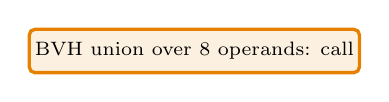
\begin{tikzpicture}
      \node[call] (u) at (0,0) {BVH union over 8 operands: call};
    \end{tikzpicture}};
  \node[font=\scriptsize, anchor=west] at ($(P1.east)+(0.2,0.15)$) {the blurred operand's program};
  \node[font=\scriptsize, anchor=west, text=black!60] at ($(P1.east)+(0.2,-0.2)$) {fresh stacks: nothing of level 0's is on them};

  % ── Level 2: one program per union operand.
  \foreach \i/\x in {1/2.9, 2/5.9, 3/8.9} {
    \node[prog] (Q\i) at (\x,5.4) {%
      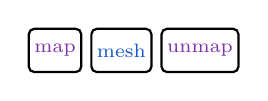
\begin{tikzpicture}
        \node[clause, text=cop] (m) at (0,0) {map};
        \node[clause, text=cleaf, right=1mm of m] (s) {mesh};
        \node[clause, text=cop, right=1mm of s] {unmap};
      \end{tikzpicture}};
    \node[font=\scriptsize, anchor=north] at ($(Q\i.south)+(0,-0.02)$) {part$_\i$};
  }
  \node[font=\large] at (10.95,5.4) {$\cdots$};
  \node[prog] (Q8) at (13.0,5.4) {%
    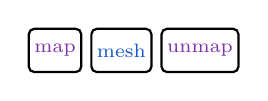
\begin{tikzpicture}
      \node[clause, text=cop] (m) at (0,0) {map};
      \node[clause, text=cleaf, right=1mm of m] (s) {mesh};
      \node[clause, text=cop, right=1mm of s] {unmap};
    \end{tikzpicture}};
  \node[font=\scriptsize, anchor=north] at ($(Q8.south)+(0,-0.02)$) {part$_8$};

  % ── Calls.
  \draw[callarrow] ($(P0.south)+(0.0,0.05)$) -- node[font=\scriptsize, right, text=black] {27 calls, one per blur tap} ($(P1.north)+(0.0,-0.05)$);
  \foreach \i in {1,2,3,8} {
    \draw[callarrow] ($(P1.south)+(0,0.05)$) -- ($(Q\i.north)+(0,0.15)$);
  }
  \node[font=\scriptsize, anchor=west, text width=2.6cm, align=left] at (14.6,5.4) {one call per operand the BVH does not prune};

  % ── Where depth counts from.
\end{tikzpicture}

\end{document}
